\chapter{Project Description}
\section*{Project Title}
Impact of climate change on the landscape of the dairy sector in Switzerland over the past decades

\section*{Description}

Climate change, as a consequence of anthropogenic greenhouse gas emissions and global population growth has become major challenge for humanity. The global increase in temperature and humidity amplifies local impact on livestock husbandry. Heat stress (HS) is defined as body hyperthermia in mammals due to excessive heat loads that cannot be sufficiently dissipated. Modern dairy cows are more susceptible to HS due to higher metabolic activity during lactation compared to other animals.

\vspace*{\baselineskip}
Based on projected growth in the human population, the global food demand is estimated to increase by 60 to 70\% by 2050 \citep{makkar_review_2018}, of which the demand for dairy products is greater than 50\% compared to the values of 2010 \citep{fao_world_2011}. Seasonal depression in milk production is mainly attributed to HS, and thereby increasing global temperatures represent a challenge to meet the growing demand for dairy products, as higher ambient temperature and humidity reduce the production efficiency of dairy cows. Climatic conditions around the world vary because animals live in a combination of environmental factors, including humidity, rainfall, wind speed, and solar radiation \citep{johnson1987}. The temperature-humidity index (THI) was proposed to represent the combined effects of ambient temperature and relative humidity associated with HS \citep{national1976livestock}. Heat stress is considered an acute effect on dairy cows when THI crosses the threshold of 72 \citep{armstrong_heat_1994} or 68 \citep{de_rensis_seasonal_2015}.

\vspace*{\baselineskip}
Heat stress causes significant economic losses to the livestock sector \citep{key_climate_2014}. For example, estimated losses in the U.S. range from \$ 1.7 to 2.4 billion, of which \$ 0.9 billion are specific to the dairy sector \citep{st-pierre_economic_2003}. Even in a temperate climatic region, such as Central Europe, dairy cows are greatly affected by seasonal exposure to heat \citep{fabris_effect_2019}. Although such financial estimates are currently not available in Switzerland, our analysis showed reductions in milk yield (MY) and milk fat and protein contents in Swiss dairy farms during the summer months, translating into significant losses in dairy food quality, nutrients, and farm sustainability (Fig.~\ref{fig:niu_annual_seasonality}).

\begin{figure}[H]
    \centering
    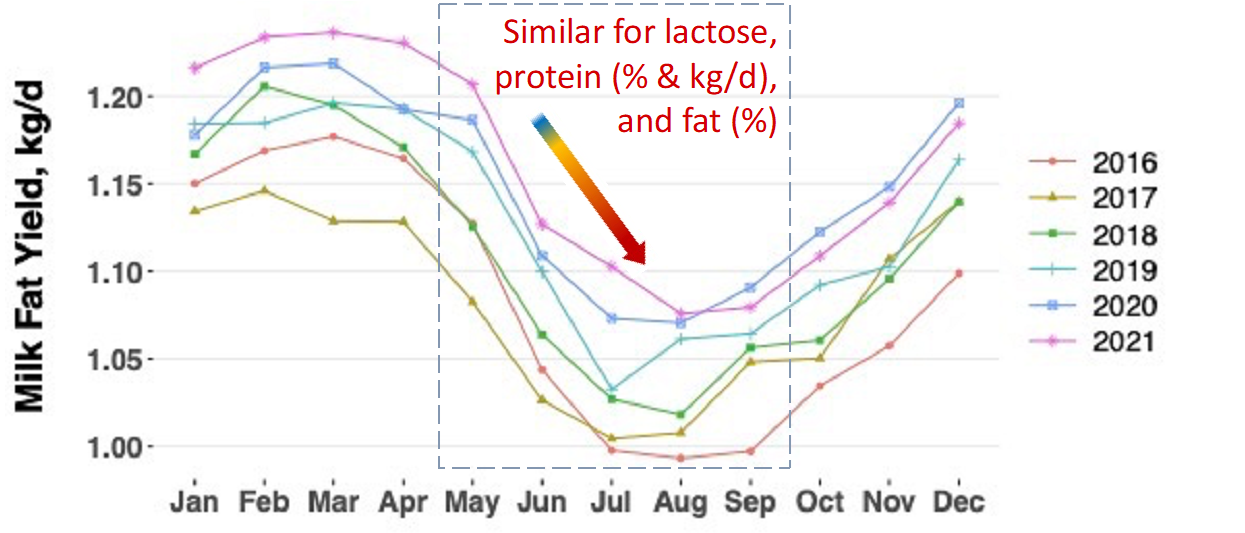
\includegraphics[width=0.7\textwidth]{./thesis/figures/project_description.png}
    \renewcommand{\thefigure}{A}
    %\captionsetup{list=false}
    \caption{Based on a total of 2'090'000 test day records from Swissherdbook, Niu et al., (unpubl.) analyzed milk fat yield of cows in registered Swiss dairy farms during 6 consecutive years across the annual cycle.}
    \label{fig:niu_annual_seasonality}
\end{figure}

Hence, our objective is to analyze, with appropriate methods, extreme weather effects on the quantitative and qualitative aspects of the dairy business in Switzerland with an unprecedented granularity level. The analysis should be performed on cow- or farm-level datasets. In addition, meteorological data from MeteoSwiss \citep{meteoswiss} allow us to investigate potential relationships between parameters at the cow level, the farm level, and the HS factors. Ideally, the work will provide valuable insights for the dairy industry, policy makers, insurances, and other stakeholders in the Swiss dairy value chain.
